%%% CAPITOLO 3

\section{Analisi di previsione}

Per la costruzione del modello di previsione ho deciso di utilizzare il modello di analisi statistica chiamato
\textbf{ARIMA}\footnote{
    \href{https://www.investopedia.com/terms/a/autoregressive-integrated-moving-average-arima.asp}{https://www.investopedia.com/terms/a/autoregressive-integrated-moving-average-arima.asp}
} (\textbf{A}uto\textbf{R}egressive \textbf{I}ntegrated \textbf{M}oving \textbf{A}verage).
Questo modello utilizza i dati delle serie temporali per permettere di capire meglio il dataset e per effettuare predizioni su trend futuri.

Questo sistema è una forma di \emph{analisi di regressione} che calcola la forza di una variabile aleatoria indipendente relativamente ai cambiamenti di altre variabili.
L'obiettivo di questo modello è di effettuare predizioni sul futuro delle securities esaminando le differenze tra i valori nelle serie temporali invece di utilizzare valori attuali.  

Possiamo evidenziare le componenti fondamentali di ARIMA scomponendo il suo acronimo:
\begin{itemize}
    \item \emph{Autoregression (AR)}: Si Riferisce ad un modello che mostra una variabile che cambia in base alla regressione
    del suo passato o dei suoi valori precedenti.
    \item \emph{Integrated (I)}: Rappresenta la differenziazione di osservazioni grezze per permettere alla serie temporale di diventare
    stazionaria. (permettendo la applicazione della auto regressione e media mobile \emph{ARMA}).
    \item \emph{Moving average (MA)}: Incorpora la dipendeza tra una osservazione ed l'errore residuo dal modelli di media 
    mobile applicato alle osservazioni passate.
\end{itemize}

Nel modello ARIMA ogni componente visto qui sopra funziona come parametro avente una notazione standard, 
un esempio di notazione standard sarebbe ARIMA con \(p, d\) e \(q\), dove valori interi sostituiscono i parametri
per indicare la tipologia del modello ARIMA utilizzato. I parametri posso essere definiti come:

\begin{itemize}
    \item \(p\): Il numero di osservazioni passate nel modello.
    \item \(d\): Il numero di volte che le osservazioni grezze sono state differenziate, chiamato anche grado di differenziazione.
    \item \(q\): la dimensione della finestra relativa alla media mobile, chiamato anche ordine della media mobile.
\end{itemize}

Impostando i parametri visti qui sopra possiamo ottenere dei \emph{casi particolari}, utili per le analisi:

\begin{itemize}
    \item \(\text{ARIMA} (0,0,0)\): Rumore bianco.
    \item \(\text{ARIMA} (0,1,0)\) senza costante: Passeggiata 
    aleatoria\footnote{
        Serie con passi in direzioni casuali, \href{https://it.wikipedia.org/wiki/Passeggiata_aleatoria}{https://it.wikipedia.org/wiki/Passeggiata\_aleatoria}
    }.
    \item \(\text{ARIMA} (p,0,q)\): \(\text{ARMA} (p,q)\).
    \item \(\text{ARIMA} (p,0,0)\): modello \(\text{AR} (p)\).
    \item \(\text{ARIMA} (0,0,q)\): modello \(\text{MA} (q)\).
    \item \(\text{ARIMA} (0,1,2)\): modello "smorzato" di 
    Holt.\footnote{
        \href{https://otexts.com/fpp3/holt.html}{https://otexts.com/fpp3/holt.html}
    }
    \item \(\text{ARIMA} (0,1,1)\): senza costante: modello SES.
    \item \(\text{ARIMA} (0,2,2)\): metodo lineare di Holt\footnotemark[28], con errori aggiuntivi.
\end{itemize}

Una delle più note debolezze del modello ARIMA nel contesto finanziario è la inabilità di catturare il clustering della volatilità
che si osserva nella maggior parte degli asset finanziari.

Per questo progetto al fine di identificare i parametri migliori \(p, d \text{ e } q \) da applicare è stata utilizzata la libreria 
\emph{pmdarima}\footnote{
    \href{http://alkaline-ml.com/pmdarima/1.8.3/about.html}{http://alkaline-ml.com/pmdarima/1.8.3/about.html}
}, che grazie alla funzione \verb|auto_arima| mediante una ricerca a griglia riesce a trovare valori che minimizzano il valore 
\verb|AIC|\footnote{
    Stimatore per gli errori di predizione, \href{https://en.wikipedia.org/wiki/Akaike_information_criterion}{https://en.wikipedia.org/wiki/Akaike\_information\_criterion}
}.

\subsection{Modello di previsione per Meta (FB)}

Per Meta, è stato identificato come valore dei parametri migliore \(p=3, d=1, q=1\) con un errore \verb|AIC| pari a \(1836.767\) (figura \ref{fig:fb_arima_param}).

\begin{figure}[ht]
    \centering
    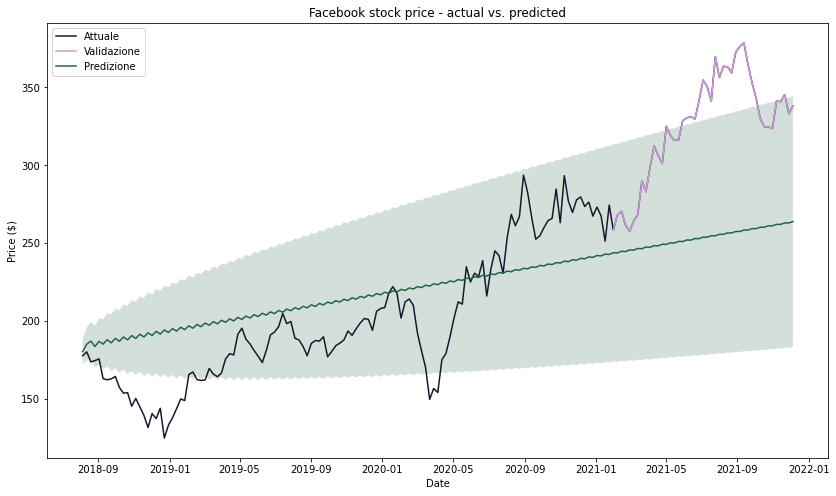
\includegraphics[width=0.8\textwidth]{fb_arima_pred.png}
    \caption{Predizione sul prezzo di FB usando ARIMA}
    \label{fig:fb_arima_pred}
\end{figure}

Dalla predizione a figura \ref{fig:fb_arima_pred} si nota che data la alta volatilità del titolo ci sono stati momenti dove il prezzo predetto è stato molto lontano da quello reale,
come per esempio nel 2018 o verso la fine nell'anno del 2021.
Tuttavia nel periodo centrale la predizione è stata sempre abbastanza vicina al prezzo predetto, rimanendo nell'intervallo di confidenza.\\
A figura \ref{fig:fb_arima_val} si può prendere visione a cadenza mensile nel periodo finale di 10 mesi la differenza tra il prezzo reale e quello predetto, si nota come sia molto distante il vero prezzo a causa della elevata volatilità.

\begin{figure}[ht]
    \centering
    \begin{minipage}{.5\textwidth}
        \centering
        \vspace{1.68cm}
        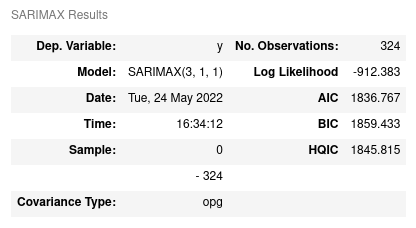
\includegraphics[width=1\linewidth]{fb_arima_par.png}
        \captionof{figure}{Parametri di ARIMA identificati per FB}
        \label{fig:fb_arima_param}
    \end{minipage}%
    \begin{minipage}{.5\textwidth}
        \centering
        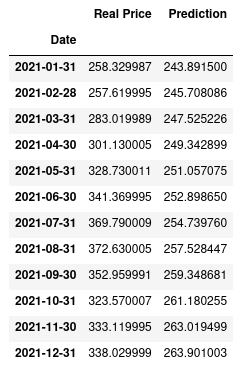
\includegraphics[width=.5\linewidth]{fb_arima_val.png}
        \captionof{figure}{Prezzo reale vs predizione FB}
        \label{fig:fb_arima_val}
    \end{minipage}
\end{figure}

\pagebreak

\subsection{Modello di previsione per Alphabet (GOOG)}

Per Alphabet, è stato identificato come valore dei parametri migliore \(p=3, d=1, q=2\) con un errore \verb|AIC| pari a \(3107.301\) (figura \ref{fig:goog_arima_param}).

\begin{figure}[ht]
    \centering
    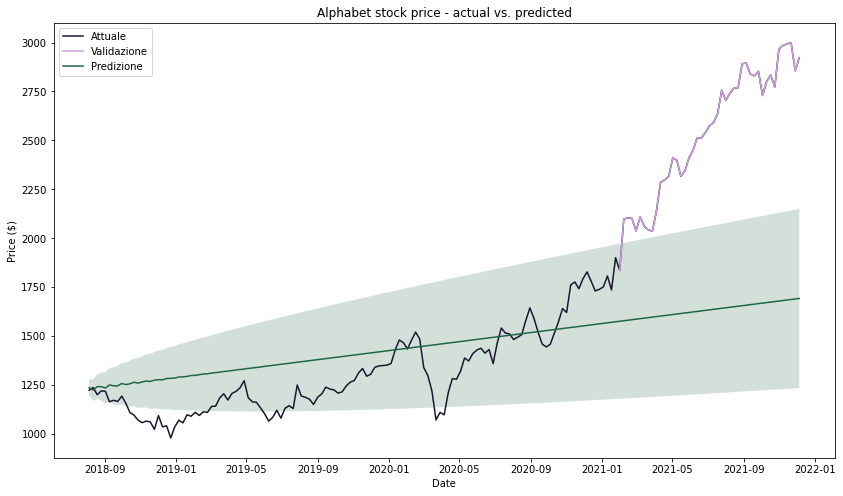
\includegraphics[width=0.8\textwidth]{goog_arima_pred.png}
    \caption{Predizione sul prezzo di GOOG usando ARIMA}
    \label{fig:goog_arima_pred}
\end{figure}

Dal grafico di predizione a figura \ref{fig:goog_arima_pred} si nota come il prezzo predetto sia stato vicino a quello reale solo nella parte centrale del grafico, verso la fine a causa della elevata volatilità si nota
come il prezzi si sia distaccato enormemente.
Analizzando la tabella a figura \ref{fig:goog_arima_val} con il prezzo reale e quello predetto nel periodo di valutazione si può notare come la differenza sia parecchio elevata, rendendo evidente le debolezze di questo modello statistico.

\begin{figure}[ht]
    \centering
    \begin{minipage}{.5\textwidth}
        \centering
        \vspace{2cm}
        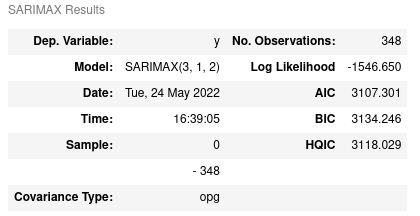
\includegraphics[width=1\linewidth]{goog_arima_par.png}
        \captionof{figure}{Parametri di ARIMA identificati per GOOG}
        \label{fig:goog_arima_param}
    \end{minipage}%
    \begin{minipage}{.5\textwidth}
        \centering
        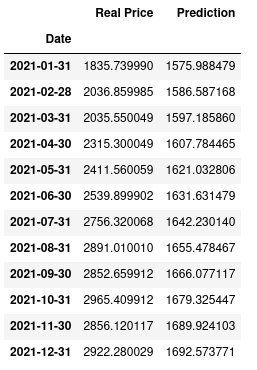
\includegraphics[width=.5\linewidth]{goog_arima_val.png}
        \captionof{figure}{Prezzo reale vs predizione GOOG}
        \label{fig:goog_arima_val}
    \end{minipage}
\end{figure}

\pagebreak

\subsection{Modello di previsione per Raytheon (rtx)}

Per Raytheon, è stato identificato come valore dei parametri migliore \(p=1, d=1, q=1\) con un errore \verb|AIC| pari a \(1201.826\) (figura \ref{fig:rtx_arima_param}).

\begin{figure}[ht]
    \centering
    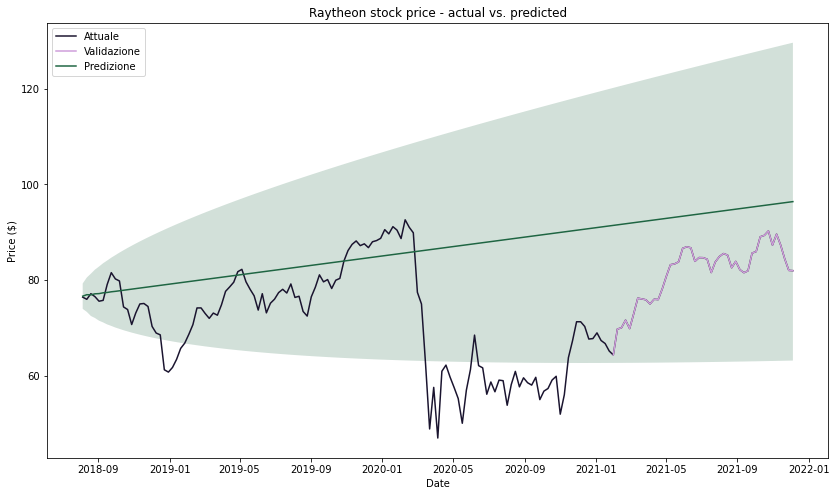
\includegraphics[width=0.8\textwidth]{rtx_arima_pred.png}
    \caption{Predizione sul prezzo di RTX usando ARIMA}
    \label{fig:rtx_arima_pred}
\end{figure}

Nel caso di RTX si nota dal grafico a figura \ref{fig:rtx_arima_pred} come nel primo periodo il prezzo predetto è stato simile a quello reale, tuttavia dal 2020 si è visto un improvviso distaccamento,
causato presumibilmente dalla crisi finanziaria del 2020, verso il 2021 nel periodo di validazione si è notato come dimostrato dalla tabella a figura \ref{fig:rtx_arima_val} che il prezzo è tornato ad avvicinarsi al quello predetto.

\begin{figure}[ht]
    \centering
    \begin{minipage}{.5\textwidth}
        \centering
        \vspace{2.4cm}
        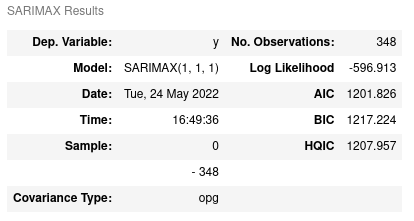
\includegraphics[width=1\linewidth]{rtx_arima_par.png}
        \captionof{figure}{Parametri di ARIMA identificati per RTX}
        \label{fig:rtx_arima_param}
    \end{minipage}%
    \begin{minipage}{.5\textwidth}
        \centering
        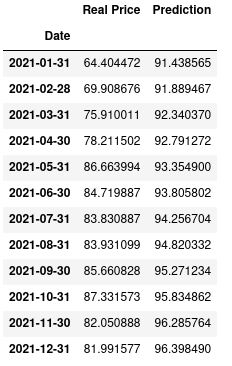
\includegraphics[width=.5\linewidth]{rtx_arima_val.png}
        \captionof{figure}{Prezzo reale vs predizione RTX}
        \label{fig:rtx_arima_val}
    \end{minipage}
\end{figure}

\pagebreak

\subsection{Modello di previsione per Lockheed Martin (LMT)}

Per Lockheed Martin, è stato identificato come valore dei parametri migliore \(p=0, d=1, q=2\) con un errore \verb|AIC| pari a \(1996.251\) (figura \ref{fig:lmt_arima_param}).

\begin{figure}[ht]
    \centering
    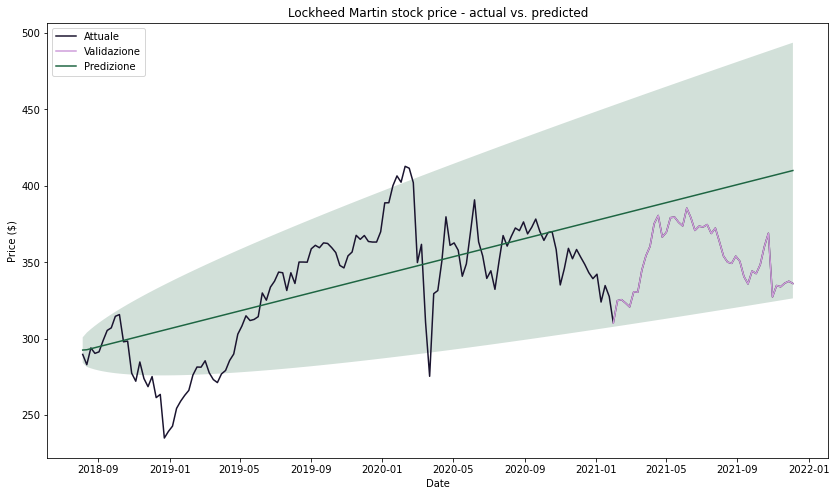
\includegraphics[width=0.8\textwidth]{lmt_arima_pred.png}
    \caption{Predizione sul prezzo di LMT usando ARIMA}
    \label{fig:lmt_arima_pred}
\end{figure}

Nel grafico di predizione a figura \ref{fig:lmt_arima_pred} è reso evidente come in alcuni momenti la predizione sul prezzo è stata vicina a quello reale, seppur ci sono stati due momenti dove il prezzo è uscito
dall'intervallo di confidenza.
Dalla tabella a figura \ref{fig:lmt_arima_val} si può notare nel periodo di validazione come il prezzo verso la metà si è avvicinato a quello predetto.

\begin{figure}[ht]
    \centering
    \begin{minipage}{.5\textwidth}
        \centering
        \vspace{2.21cm}
        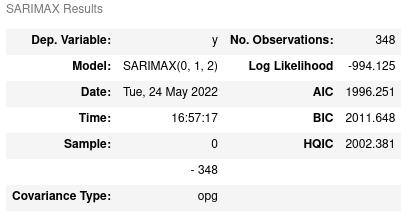
\includegraphics[width=1\linewidth]{lmt_arima_par.png}
        \captionof{figure}{Parametri di ARIMA identificati per LMT}
        \label{fig:lmt_arima_param}
    \end{minipage}%
    \begin{minipage}{.5\textwidth}
        \centering
        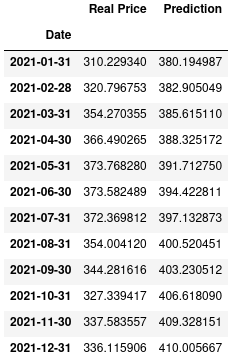
\includegraphics[width=.5\linewidth]{lmt_arima_val.png}
        \captionof{figure}{Prezzo reale vs predizione LMT}
        \label{fig:lmt_arima_val}
    \end{minipage}
\end{figure}

\pagebreak

\subsection{Modello di previsione per Bank of America (BAC)}\

Per Bank of America, è stato identificato come valore dei parametri migliore \(p=1, d=1, q=1\) con un errore \verb|AIC| pari a \(584.994\) (figura \ref{fig:bac_arima_param}).

\begin{figure}[ht]
    \centering
    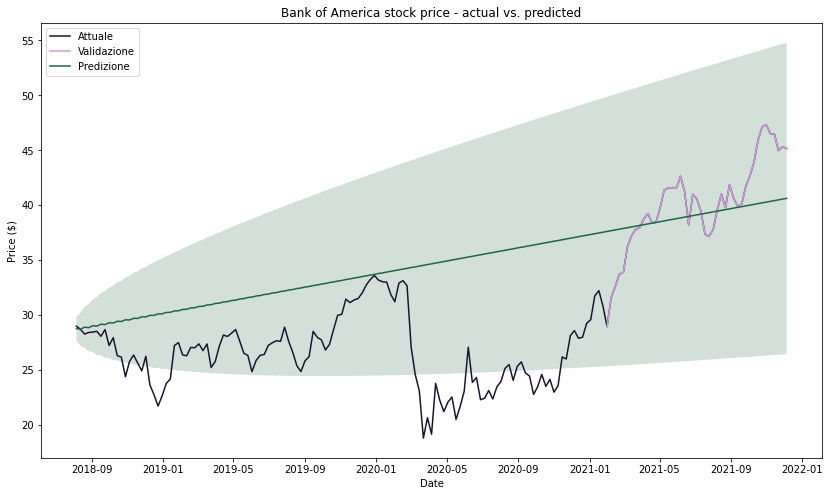
\includegraphics[width=0.8\textwidth]{bac_arima_pred.png}
    \caption{Predizione sul prezzo di BAC usando ARIMA}
    \label{fig:bac_arima_pred}
\end{figure}

Nel grafico a figura \ref{fig:bac_arima_pred} viene evidenziato come la predizione è stata vicina al prezzo reale nel periodo 2019-2020, successivamente c'è stato un grosso distacco sempre
come visto precedentemente a causa della crisi finanziaria del 2020. verso il 2021 nel periodo di validazione come evidenziato dalla tabella a figura \ref{fig:bac_arima_val}, il prezzo si è avvicinato a quello predetto, rimanendo sempre
nell'intervallo di confidenza.

\begin{figure}[ht]
    \centering
    \begin{minipage}{.5\textwidth}
        \centering
        \vspace{2.21cm}
        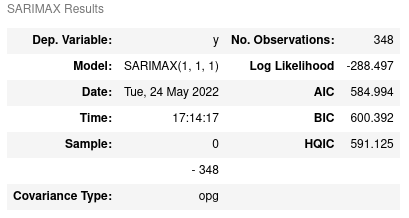
\includegraphics[width=1\linewidth]{bac_arima_par.png}
        \captionof{figure}{Parametri di ARIMA identificati per BAC}
        \label{fig:bac_arima_param}
    \end{minipage}%
    \begin{minipage}{.5\textwidth}
        \centering
        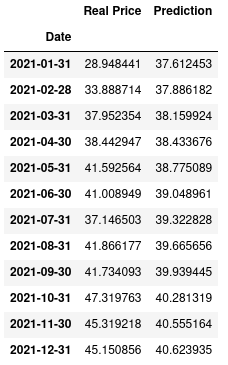
\includegraphics[width=.5\linewidth]{bac_arima_val.png}
        \captionof{figure}{Prezzo reale vs predizione BAC}
        \label{fig:bac_arima_val}
    \end{minipage}
\end{figure}

\pagebreak

\subsection{Modello di previsione per JPMorgan Chase (JPM)}\

Per Bank of America, è stato identificato come valore dei parametri migliore \(p=0, d=1, q=0\) (caso particolare di ARIMA) con un errore \verb|AIC| pari a \(1336.117\) (figura \ref{fig:jpm_arima_param}).

\begin{figure}[ht]
    \centering
    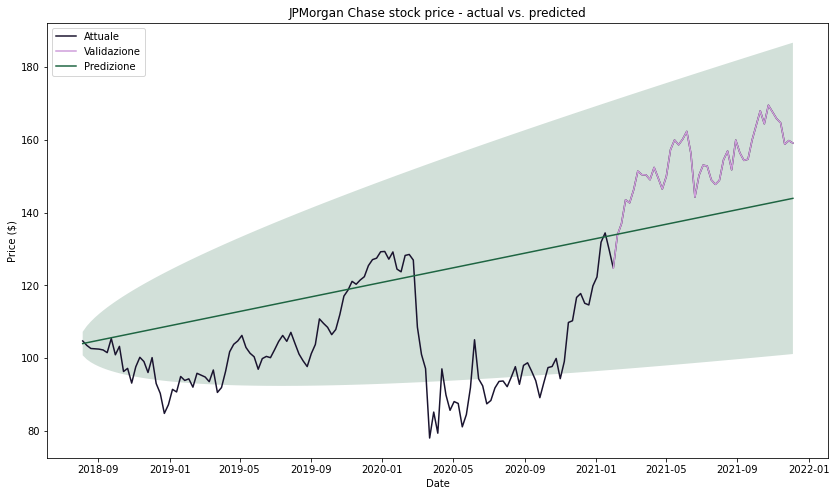
\includegraphics[width=0.8\textwidth]{jpm_arima_pred.png}
    \caption{Predizione sul prezzo di JPM usando ARIMA}
    \label{fig:jpm_arima_pred}
\end{figure}

Il grafico a figura \ref{fig:jpm_arima_pred} si comporta in maniera molto simile a ciò che è stato visto per BAC, tale comportamento si può attribuire alla correlazione
veramente alta tra i due titoli. Nella tabella a figura \ref{fig:jpm_arima_val}, si può vedere come nel periodo di verifica il prezzo sia sempre stato abbastanza vicino a quello predetto, e sempre 
nell'intervallo di confidenza (in maniera simile a BAC).

\begin{figure}[ht]
    \centering
    \begin{minipage}{.5\textwidth}
        \centering
        \vspace{2.21cm}
        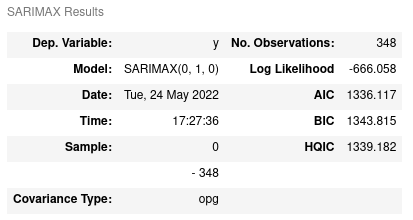
\includegraphics[width=1\linewidth]{jpm_arima_par.png}
        \captionof{figure}{Parametri di ARIMA identificati per JPM}
        \label{fig:jpm_arima_param}
    \end{minipage}%
    \begin{minipage}{.5\textwidth}
        \centering
        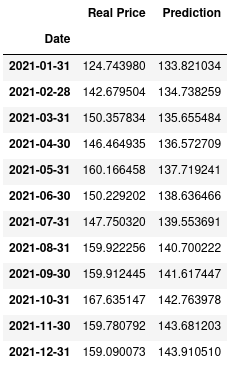
\includegraphics[width=.5\linewidth]{jpm_arima_val.png}
        \captionof{figure}{Prezzo reale vs predizione JPM}
        \label{fig:jpm_arima_val}
    \end{minipage}
\end{figure}

\pagebreak